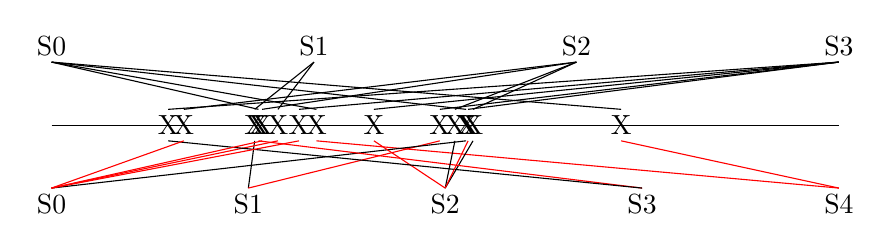
\begin{tikzpicture}
\draw [thin] (0,0) -- (10.0,0);
\node at (0.0, 1) {S0};
\node at (3.3333333333333335, 1) {S1};
\node at (6.666666666666667, 1) {S2};
\node at (10.0, 1) {S3};
\node at (0.0, -1) {S0};
\node at (2.5, -1) {S1};
\node at (5.0, -1) {S2};
\node at (7.5, -1) {S3};
\node at (10.0, -1) {S4};
\node at  (3.364992044479047,0) {X};
\draw (3.364992044479047, 0.2) -- (0.0, 0.8);
\draw[red] (3.364992044479047,-0.2) -- (10.0, -0.8);
\node at  (2.5803335400550615,0) {X};
\draw (2.5803335400550615, 0.2) -- (3.3333333333333335, 0.8);
\draw (2.5803335400550615,-0.2) -- (2.5, -0.8);
\node at  (2.875688779130253,0) {X};
\draw (2.875688779130253, 0.2) -- (3.3333333333333335, 0.8);
\draw[red] (2.875688779130253,-0.2) -- (0.0, -0.8);
\node at  (4.931675709140759,0) {X};
\draw (4.931675709140759, 0.2) -- (10.0, 0.8);
\draw[red] (4.931675709140759,-0.2) -- (2.5, -0.8);
\node at  (5.264693287491485,0) {X};
\draw (5.264693287491485, 0.2) -- (0.0, 0.8);
\draw (5.264693287491485,-0.2) -- (0.0, -0.8);
\node at  (5.353130965881627,0) {X};
\draw (5.353130965881627, 0.2) -- (6.666666666666667, 0.8);
\draw (5.353130965881627,-0.2) -- (5.0, -0.8);
\node at  (4.094297360184821,0) {X};
\draw (4.094297360184821, 0.2) -- (10.0, 0.8);
\draw[red] (4.094297360184821,-0.2) -- (5.0, -0.8);
\node at  (2.6283261310021997,0) {X};
\draw (2.6283261310021997, 0.2) -- (0.0, 0.8);
\draw[red] (2.6283261310021997,-0.2) -- (7.5, -0.8);
\node at  (1.4820897156520827,0) {X};
\draw (1.4820897156520827, 0.2) -- (10.0, 0.8);
\draw (1.4820897156520827,-0.2) -- (7.5, -0.8);
\node at  (5.123353286558451,0) {X};
\draw (5.123353286558451, 0.2) -- (6.666666666666667, 0.8);
\draw (5.123353286558451,-0.2) -- (5.0, -0.8);
\node at  (3.1434151863461772,0) {X};
\draw (3.1434151863461772, 0.2) -- (10.0, 0.8);
\draw[red] (3.1434151863461772,-0.2) -- (0.0, -0.8);
\node at  (7.234570928677267,0) {X};
\draw (7.234570928677267, 0.2) -- (0.0, 0.8);
\draw[red] (7.234570928677267,-0.2) -- (10.0, -0.8);
\node at  (5.29070505110373,0) {X};
\draw (5.29070505110373, 0.2) -- (10.0, 0.8);
\draw[red] (5.29070505110373,-0.2) -- (5.0, -0.8);
\node at  (2.6749324041594247,0) {X};
\draw (2.6749324041594247, 0.2) -- (6.666666666666667, 0.8);
\draw[red] (2.6749324041594247,-0.2) -- (0.0, -0.8);
\node at  (1.6802892292761933,0) {X};
\draw (1.6802892292761933, 0.2) -- (6.666666666666667, 0.8);
\draw[red] (1.6802892292761933,-0.2) -- (0.0, -0.8);
\end{tikzpicture}
%--------------
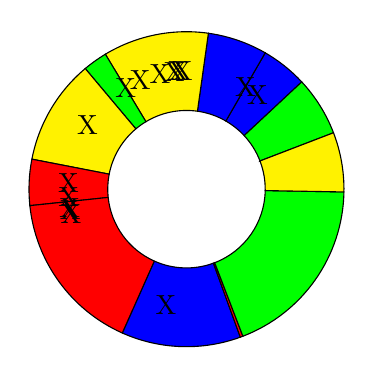
\begin{tikzpicture}
\draw[fill=green] (21:1cm) arc [start angle = 21, end angle=43, radius=1cm] --++(43:1cm) arc  [start angle = 43, end angle=21, radius=2cm] --++(21:-1cm)--cycle;
\draw[fill=blue] (43:1cm) arc [start angle = 43, end angle=60, radius=1cm] --++(60:1cm) arc  [start angle = 60, end angle=43, radius=2cm] --++(43:-1cm)--cycle;
\draw[fill=blue] (60:1cm) arc [start angle = 60, end angle=82, radius=1cm] --++(82:1cm) arc  [start angle = 82, end angle=60, radius=2cm] --++(60:-1cm)--cycle;
\draw[fill=yellow] (82:1cm) arc [start angle = 82, end angle=121, radius=1cm] --++(121:1cm) arc  [start angle = 121, end angle=82, radius=2cm] --++(82:-1cm)--cycle;
\draw[fill=green] (121:1cm) arc [start angle = 121, end angle=130, radius=1cm] --++(130:1cm) arc  [start angle = 130, end angle=121, radius=2cm] --++(121:-1cm)--cycle;
\draw[fill=yellow] (130:1cm) arc [start angle = 130, end angle=169, radius=1cm] --++(169:1cm) arc  [start angle = 169, end angle=130, radius=2cm] --++(130:-1cm)--cycle;
\draw[fill=red] (169:1cm) arc [start angle = 169, end angle=186, radius=1cm] --++(186:1cm) arc  [start angle = 186, end angle=169, radius=2cm] --++(169:-1cm)--cycle;
\draw[fill=red] (186:1cm) arc [start angle = 186, end angle=246, radius=1cm] --++(246:1cm) arc  [start angle = 246, end angle=186, radius=2cm] --++(186:-1cm)--cycle;
\draw[fill=blue] (246:1cm) arc [start angle = 246, end angle=290, radius=1cm] --++(290:1cm) arc  [start angle = 290, end angle=246, radius=2cm] --++(246:-1cm)--cycle;
\draw[fill=red] (290:1cm) arc [start angle = 290, end angle=291, radius=1cm] --++(291:1cm) arc  [start angle = 291, end angle=290, radius=2cm] --++(290:-1cm)--cycle;
\draw[fill=green] (291:1cm) arc [start angle = 291, end angle=359, radius=1cm] --++(359:1cm) arc  [start angle = 359, end angle=291, radius=2cm] --++(291:-1cm)--cycle;
\draw[fill=yellow] (21:1cm) arc [start angle = 21, end angle=-1, radius=1cm] --++(-1:1cm) arc  [start angle = -1, end angle=21, radius=2cm] --++(21:-1cm)--cycle;
\node at ({121}:1.5cm) {X};
\node at ({92}:1.5cm) {X};
\node at ({103}:1.5cm) {X};
\node at ({177}:1.5cm) {X};
\node at ({189}:1.5cm) {X};
\node at ({192}:1.5cm) {X};
\node at ({147}:1.5cm) {X};
\node at ({94}:1.5cm) {X};
\node at ({53}:1.5cm) {X};
\node at ({184}:1.5cm) {X};
\node at ({113}:1.5cm) {X};
\node at ({260}:1.5cm) {X};
\node at ({190}:1.5cm) {X};
\node at ({96}:1.5cm) {X};
\node at ({60}:1.5cm) {X};
\end{tikzpicture}
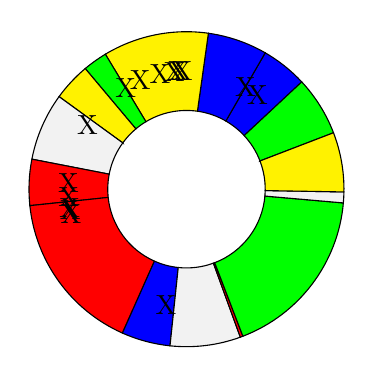
\begin{tikzpicture}
\draw[fill=green] (21:1cm) arc [start angle = 21, end angle=43, radius=1cm] --++(43:1cm) arc  [start angle = 43, end angle=21, radius=2cm] --++(21:-1cm)--cycle;
\draw[fill=blue] (43:1cm) arc [start angle = 43, end angle=60, radius=1cm] --++(60:1cm) arc  [start angle = 60, end angle=43, radius=2cm] --++(43:-1cm)--cycle;
\draw[fill=blue] (60:1cm) arc [start angle = 60, end angle=82, radius=1cm] --++(82:1cm) arc  [start angle = 82, end angle=60, radius=2cm] --++(60:-1cm)--cycle;
\draw[fill=yellow] (82:1cm) arc [start angle = 82, end angle=121, radius=1cm] --++(121:1cm) arc  [start angle = 121, end angle=82, radius=2cm] --++(82:-1cm)--cycle;
\draw[fill=green] (121:1cm) arc [start angle = 121, end angle=130, radius=1cm] --++(130:1cm) arc  [start angle = 130, end angle=121, radius=2cm] --++(121:-1cm)--cycle;
\draw[fill=yellow] (130:1cm) arc [start angle = 130, end angle=144, radius=1cm] --++(144:1cm) arc  [start angle = 144, end angle=130, radius=2cm] --++(130:-1cm)--cycle;
\draw[fill=gray!10] (144:1cm) arc [start angle = 144, end angle=169, radius=1cm] --++(169:1cm) arc  [start angle = 169, end angle=144, radius=2cm] --++(144:-1cm)--cycle;
\draw[fill=red] (169:1cm) arc [start angle = 169, end angle=186, radius=1cm] --++(186:1cm) arc  [start angle = 186, end angle=169, radius=2cm] --++(169:-1cm)--cycle;
\draw[fill=red] (186:1cm) arc [start angle = 186, end angle=246, radius=1cm] --++(246:1cm) arc  [start angle = 246, end angle=186, radius=2cm] --++(186:-1cm)--cycle;
\draw[fill=blue] (246:1cm) arc [start angle = 246, end angle=264, radius=1cm] --++(264:1cm) arc  [start angle = 264, end angle=246, radius=2cm] --++(246:-1cm)--cycle;
\draw[fill=gray!10] (264:1cm) arc [start angle = 264, end angle=290, radius=1cm] --++(290:1cm) arc  [start angle = 290, end angle=264, radius=2cm] --++(264:-1cm)--cycle;
\draw[fill=red] (290:1cm) arc [start angle = 290, end angle=291, radius=1cm] --++(291:1cm) arc  [start angle = 291, end angle=290, radius=2cm] --++(290:-1cm)--cycle;
\draw[fill=green] (291:1cm) arc [start angle = 291, end angle=355, radius=1cm] --++(355:1cm) arc  [start angle = 355, end angle=291, radius=2cm] --++(291:-1cm)--cycle;
\draw[fill=gray!10] (355:1cm) arc [start angle = 355, end angle=359, radius=1cm] --++(359:1cm) arc  [start angle = 359, end angle=355, radius=2cm] --++(355:-1cm)--cycle;
\draw[fill=yellow] (21:1cm) arc [start angle = 21, end angle=-1, radius=1cm] --++(-1:1cm) arc  [start angle = -1, end angle=21, radius=2cm] --++(21:-1cm)--cycle;
\node at ({121}:1.5cm) {X};
\node at ({92}:1.5cm) {X};
\node at ({103}:1.5cm) {X};
\node at ({177}:1.5cm) {X};
\node at ({189}:1.5cm) {X};
\node at ({192}:1.5cm) {X};
\node at ({147}:1.5cm) {X};
\node at ({94}:1.5cm) {X};
\node at ({53}:1.5cm) {X};
\node at ({184}:1.5cm) {X};
\node at ({113}:1.5cm) {X};
\node at ({260}:1.5cm) {X};
\node at ({190}:1.5cm) {X};
\node at ({96}:1.5cm) {X};
\node at ({60}:1.5cm) {X};
\end{tikzpicture}
